\documentclass[a4paper,10pt]{scrartcl}
\usepackage[utf8]{inputenc}

% Title Page
\title{Computer Modeling and Finite Difference Methods}
\author{Andrew D. Wickert}
\date{Last updated \today}

\usepackage{listings}
\usepackage{framed}

\usepackage{amssymb}
\usepackage{amsmath}
\usepackage{graphicx}
\lstset{mathescape,basicstyle=\ttfamily} % Allow escaping to LaTeX inside $..$

\usepackage{color}
\usepackage[hyphens]{url}
\usepackage[colorlinks=true]{hyperref}
\usepackage[T1]{fontenc}

\newcommand{\todo}[1]{\textcolor{red}{@TODO: #1}} 
 
% From http://en.wikibooks.org/wiki/LaTeX/Source_Code_Listings, modified a little

\definecolor{mygreen}{rgb}{0,0.6,0}
\definecolor{mygray}{rgb}{0.5,0.5,0.5}
\definecolor{mymauve}{rgb}{0.58,0,0.82}

\lstset{ %
  backgroundcolor=\color{white},   % choose the background color; you must add \usepackage{color} or \usepackage{xcolor}
  basicstyle=\scriptsize,          % the size of the fonts that are used for the code
  breakatwhitespace=false,         % sets if automatic breaks should only happen at whitespace
  breaklines=true,                 % sets automatic line breaking
  captionpos=b,                    % sets the caption-position to bottom
  commentstyle=\color{mygreen},    % comment style
  deletekeywords={...},            % if you want to delete keywords from the given language
  escapeinside={\%*}{*)},          % if you want to add LaTeX within your code
  extendedchars=true,              % lets you use non-ASCII characters; for 8-bits encodings only, does not work with UTF-8
  frame=single,                    % adds a frame around the code
  keepspaces=true,                 % keeps spaces in text, useful for keeping indentation of code (possibly needs columns=flexible)
  keywordstyle=\color{blue},       % keyword style
  language=Python,                 % the language of the code
  morekeywords={*,...},            % if you want to add more keywords to the set
  numbers=left,                    % where to put the line-numbers; possible values are (none, left, right)
  numbersep=5pt,                   % how far the line-numbers are from the code
  numberstyle=\tiny\color{mygray}, % the style that is used for the line-numbers
  rulecolor=\color{black},         % if not set, the frame-color may be changed on line-breaks within not-black text (e.g. comments (green here))
  showspaces=false,                % show spaces everywhere adding particular underscores; it overrides 'showstringspaces'
  showstringspaces=false,          % underline spaces within strings only
  showtabs=false,                  % show tabs within strings adding particular underscores
  stepnumber=2,                    % the step between two line-numbers. If it's 1, each line will be numbered
  stringstyle=\color{mymauve},     % string literal style
  tabsize=2,                       % sets default tabsize to 2 spaces
  title=\lstname                   % show the filename of files included with \lstinputlisting; also try caption instead of title
}

\begin{document}
\maketitle

\section{Philosophy of Computer Modeling}

Before starting to write a program to solve a problem, one must ask oneself important questions such as,
\begin{itemize}
 \item Why do I want to model this system?
 \begin{itemize}
  \item To test relationships between variables and gain some new physical insight that would be difficult to attain with reasoning or analytical solutions alone?
  \item To accurately represent a real physical system, including efforts to try to match data and their associated uncertainties?
  \item To make a prediction of the future and/or past?
  \item Other?
 \end{itemize}
 \item What is the best way to model it?
 \begin{itemize}
  \item As a set of continuum equations?
  \item As a number of individual agents that take actions in their virtual environment?
  \item With full-realism physics or simplified rules?
  \item Other?
 \end{itemize}
 \item Should I wish to, how do I compare the ``real world'' and the data? Or perhaps improve the fit between data and model?
\end{itemize}

\begin{framed}
\noindent\textbf{The first algorithm}

The first computer program was written in 1843 (or maybe 1842) by Lady Ada Lovelace, with a numerical method to calculate the Bernoulli Numbers. She was 28!
\end{framed}

\section{Mathematics Review}

\subsection{Vectors}

A vector is a one-dimensional matrix. It is thus a special case of the more general class of matrices. It may be a row,
\begin{equation}
\vec{a} =
 \begin{bmatrix}
  a_{1} & a_{2} & \cdots & a_{n} \\
 \end{bmatrix},
\end{equation}
or a column,
\begin{equation}
\vec{a} =
 \begin{bmatrix}
  a_{1} \\
  a_{2} \\
  \vdots \\
  a_{m}
 \end{bmatrix}.
\end{equation}

Vectors can define a direction. For example, in three dimensions:
\begin{equation}
\vec{r} =
 \begin{bmatrix}
  x \\
  y \\
  z
 \end{bmatrix}.
\end{equation}

In addition to the top arrow notation, a boldface (but italicized) notation is also common for vectors:
\begin{equation}
\vec{a} = \boldsymbol{a}
\end{equation}


\subsection{Two-dimensional matrices}

A two-dimensional matrix of $m$ rows and $n$ columns can be represented in a way that is an extension of our vector notation; these are represented by boldface Roman (non-italic) characters. They are often, but not always, represented by capital letters:
\begin{equation}
\mathbf{A} =
 \begin{bmatrix}
  a_{1,1} & a_{1,2} & \cdots & a_{1,n} \\
  a_{2,1} & a_{2,2} & \cdots & a_{2,n} \\
  \vdots & \vdots & \ddots & \vdots \\
  a_{m,1} & a_{m,2} & \cdots & a_{m,n} \\
 \end{bmatrix}
\end{equation}

A 3$\times$3 matrix is often used to represent a \textit{tensor} that can define the orientation and dimensions in a three-dimensional shape (ellipsoid). Such a matrix can also describe stress-strain relationships, mineral symmetry, or any other material anisotropy (or isotropy, if the 3$\times$3 matrix is the identity matrix).

One special matrix is the \emph{Identity} matrix, which is an expansion of ``1'' for an array:
\begin{equation}
\mathbf{I} =
 \begin{bmatrix}
  1 & 0 & \cdots & 0 \\
  0 & 1 & \cdots & 0 \\
  \vdots & \vdots & \ddots & \vdots \\
  0 & 0 & \cdots & 1 \\
 \end{bmatrix}
\end{equation}

\subsection{Matrix operations}

\subsubsection{Matrix multiplication}

To multiply two matrices, $\mathbf{A} \times \mathbf{B}$, follow these steps:
\begin{enumerate}
 \item Multiply each number in the first column of the matrix on the left ($\mathbf{A}$) by each number in the first row of the matrix on the right ($\mathbf{B}$), in order: $\mathbf{A}_{1,1} \times \mathbf{B}_{1,1}$, $\mathbf{A}_{2,1} \times \mathbf{B}_{1,2}$, ..., $\mathbf{A}_{1,n} \times \mathbf{B}_{m,1}$. Note that in order for this to work, the number of rows in matrix $\mathbf{A}$ must equal the number of columns in matrix $\mathbf{B}$.
 \item Sum all of these products that you have just calculated.
 \item The result is the values for the resultant matrix in location (1,1).
 \item Repeat this for each row in Matrix $\mathbf{A}$ and column in Matrix $\mathbf{B}$. If the sizes of these arrays are ($m_\mathbf{A} \times n_\mathbf{A}$) and ($m_\mathbf{B} \times n_\mathbf{B}$), then your resultant array will have dimensions ($m_\mathbf{A} \times n_\mathbf{B}$).
\end{enumerate}

An example of matrix multiplication follows:

\begin{align}
 \mathbf{A} \mathbf{B} = &
 \begin{bmatrix}
  a_{1,1} & a_{1,2} & a_{1,3} \\
  a_{2,1} & a_{2,2} & a_{2,3} \\
 \end{bmatrix}
 \begin{bmatrix}
  b_{1,1} & b_{1,2} \\
  b_{2,1} & b_{2,2} \\
  b_{3,1} & b_{3,2} \\
 \end{bmatrix}
 = \\
 &
 \begin{bmatrix}
  a_{1,1} b_{1,1} + a_{1,2} b_{2,1} + a_{1,3} b_{3,1} & a_{1,1} b_{1,2} + a_{1,2} b_{2,2} + a_{1,3} b_{3,2} \\
  a_{2,1} b_{1,1} + a_{2,2} b_{2,1} + a_{2,3} b_{3,1} & 4d {2,1} b_{1,2} + a_{2,2} b_{2,2} + a_{2,3} b_{3,2} \\
 \end{bmatrix}
\end{align}

I usually think of matrix multiplication as ``over... down''. But some better memonics include ``karate... chop!'' (the ``chop'' being obviously down) and the visual way of multiplying A and B, as follows:
\begin{align}
 \mathbf{A} \mathbf{B} = &\\
 &
 \begin{bmatrix}
  b_{1,1} & b_{1,2} \\
  b_{2,1} & b_{2,2} \\
  b_{3,1} & b_{3,2} \\
 \end{bmatrix}
 \\
 \begin{bmatrix}
  a_{1,1} & a_{1,2} & a_{1,3} \\
  a_{2,1} & a_{2,2} & a_{2,3} \\
 \end{bmatrix}
 &
 \begin{bmatrix}
  \phantom{b_{3,1}} & \phantom{b_{1,3}} \\
  \phantom{b_{3,2}} & \phantom{b_{3,2}} \\
 \end{bmatrix}
\end{align}
Here, the empty matrix can be filled with the values by multiplying the rows and columns that project (on a straight line) into that cell. (Thanks to Jack for both of these.)

\subsubsection{Determinants}

The determinant of a matrix provides information that can help us with:
\begin{itemize}
 \item Systems of linear equations
 \item Matrix inversions
\end{itemize}

The determinant of a matrix, $\mathbf{A}$, is denoted:
\begin{equation}
 |\mathbf{A}|.
\end{equation}

For a 2$\times$2 matrix, the determinant is:
\begin{equation}
 \mathbf{A} = 
 \begin{vmatrix}
  a_{1,1} & a_{1,2} \\
  a_{2,1} & a_{2,2} \\
 \end{vmatrix}
 = a_{1,1} a_{2,2} - a_{1,2} a_{2,1}
\end{equation}
While I prefer to include subscripts with a single letter, this is more commonly displayed in math textbooks as:
\begin{equation}
 \begin{vmatrix}
  a & b \\
  c & d \\
 \end{vmatrix}
 = a d - b c
\end{equation}

For a 3$\times$3 matrix, one takes an additional step. I am showing the method called Laplace Expansion, because it has an easy-to-remember pattern.
\begin{equation}
 \mathbf{A} = 
 \begin{vmatrix}
  a_{1,1} & a_{1,2} & a_{1,3} \\
  a_{2,1} & a_{2,2} & a_{2,3} \\
  a_{3,1} & a_{3,2} & a_{3,3} \\
 \end{vmatrix}
 = a_{1,1}
 \begin{vmatrix}
  a_{1,2} & a_{1,3} \\
  a_{2,2} & a_{2,3} \\
 \end{vmatrix}
- a_{1,2}
 \begin{vmatrix}
  a_{1,1} & a_{1,3} \\
  a_{2,1} & a_{2,3} \\
 \end{vmatrix}
+ a_{1,3}
 \begin{vmatrix}
  a_{1,1} & a_{1,2} \\
  a_{2,1} & a_{2,2} \\
 \end{vmatrix}
\end{equation}
 
Note the pattern -- eliminate the rows and columns in straight lines from each term on one row (you may pick any row... or column, I think, though I haven't tried this), and then solve.

Following this same nested-determinant and $+, -, +, -, ...$ pattern, you can solve any determinant to an arbitrarily large matrix. But perhaps you see one reason why we have computers.


\subsubsection{Dot products}

\begin{figure}[ht!]
\begin{center}
 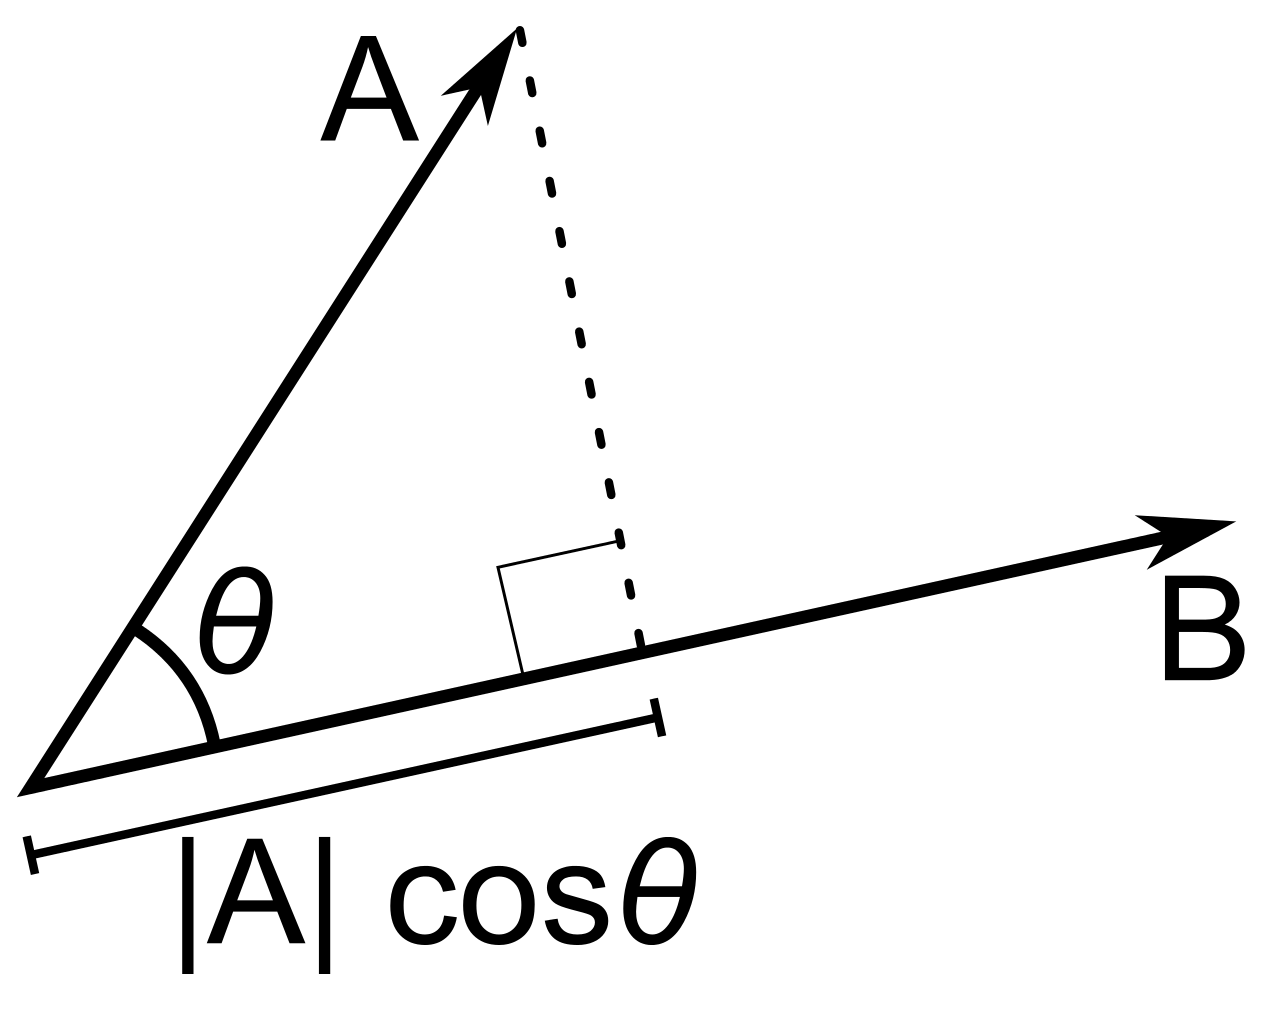
\includegraphics[width=.5\linewidth]{figures/NumericalAndMath/Dot_Product.png}
\end{center}
 \caption{The dot product can be thought of as the scalar product of the magnitude of one vector, times the magnitude of another vector that has been projected onto it. \url{https://commons.wikimedia.org/wiki/File:Dot_Product.svg}.}
\end{figure}


The dot product between two arrays can be visualized as the magnitude the product of two $n$-dimensional vectors. It is therefore also called the ``scalar product'', because it gives a scalar result.
\begin{equation}
 \vec{a} \cdot \vec{b} =
 \begin{bmatrix}
  a_{1} & a_{2} & \cdots & a_{n}
 \end{bmatrix}
 \begin{bmatrix}
  b_{1} \\
  b_{2} \\
  \vdots \\
  b_{m}
 \end{bmatrix}
 = \sum_{i=1}^{m(=n)} a_i b_i
\end{equation}

If you know the angle, $\theta_{\vec{a},\vec{b}}$, between the two vectors, a dot product can also be represented as:
\begin{equation}
 \left| \vec{a} \right|  \left| \vec{b} \right| \cos{ \left( \theta_{\vec{a},\vec{b}} \right) }
\end{equation}

\subsubsection{Cross products}

A cross product, or ``vector product'', gives the magnitude and direction of a product of two vectors, $\vec{a}$ and $\vec{b}$, where the magnitude is the area of the parallelogram created by the two vectors and the direction is given by the right-hand rule.

Cross-products are useful for:
\begin{itemize}
 \item Vector 
\end{itemize}


\begin{figure}[ht!]
\begin{center}
 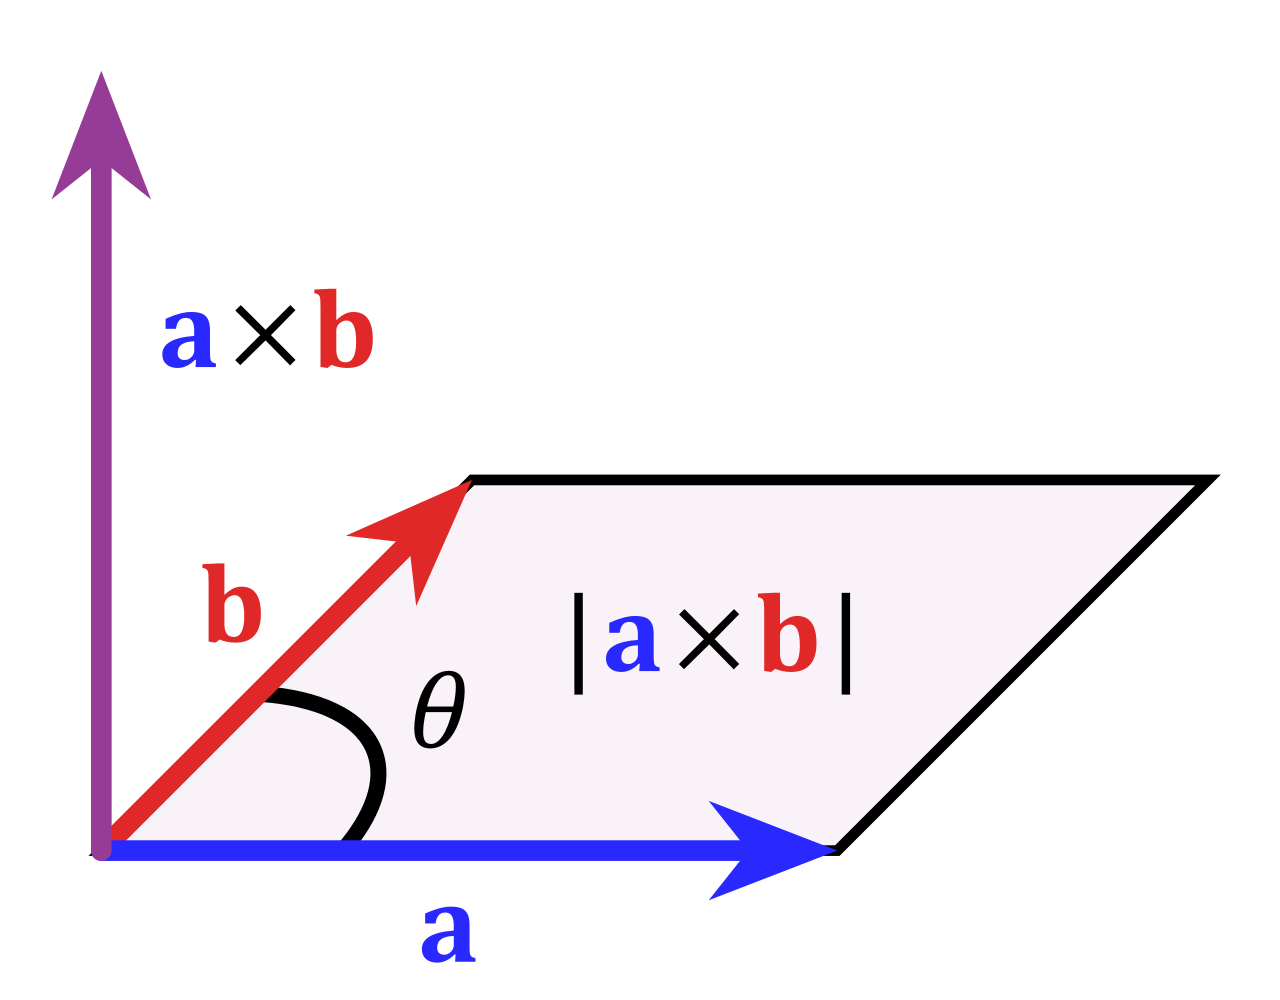
\includegraphics[width=.5\linewidth]{figures/NumericalAndMath/1280px-Cross_product_parallelogram.png}
\end{center}
 \caption{Graphical definition of the cross-product of two vectors. \url{https://commons.wikimedia.org/wiki/File:Cross_product_parallelogram.svg}.}
\end{figure}

\begin{figure}[ht!]
\begin{center}
 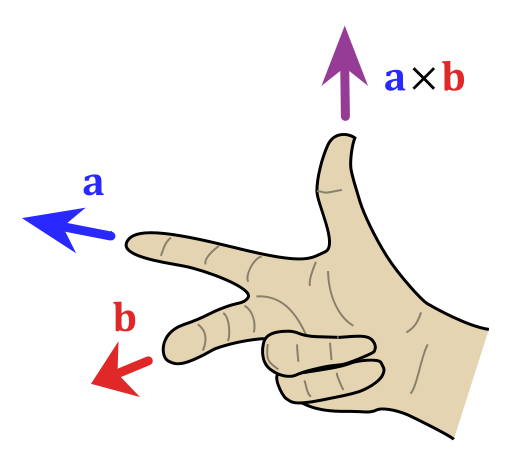
\includegraphics[width=.5\linewidth]{figures/NumericalAndMath/507px-Right_hand_rule_cross_product.png}
\end{center}
 \caption{Direction of a cross-product of vectors $\vec{a} \times \vec{b}$ as given by the right-hand rule. \url{https://commons.wikimedia.org/wiki/File:Right_hand_rule_cross_product.svg}.}
\end{figure}

The cross product can be solved in a 3-space (so for two orthogonal 2-D vectors) by solving the determinant of the following equation, here given in a 3-space ($\mathbb{R}^3$):
\begin{equation}
\vec{u} \times \vec{v} =
\begin{vmatrix}
  \hat{i}	&	\hat{j}	&	\hat{k}\\
  u_1		&	u_2	&	u_3\\
  v_1		&	v_2	&	v_3\\
\end{vmatrix}
\end{equation}


The scalar value (i.e., magnitude) of the cross product can also be obtained as follows:
\begin{equation}
\left\| \vec{a} \times \vec{b} \right\| = \left\| \vec{a} \right\| \left\| \vec{b} \right\| \sin \theta
\end{equation}

\subsubsection{Dot and cross products}

The relationship between the dot and cross products is that:
\begin{equation}
 \left\| \vec{a} \times \vec{b} \right\|^2  = \left\| \vec{a}\right\|^2  \left\|\vec{b}\right\|^2 - (\vec{a} \cdot \vec{b})^2
\end{equation}



\subsubsection{Trace}

The trace operator is given by the sum of the diagonal elements:

\begin{equation}
 \text{Tr}\left(\mathbf{A}\right) = \sum \mathbf{A} \mathbf{I}
\end{equation}


\subsubsection{Einstein notation}

\todo{}

\subsection{Derivatives}

A derivative is the change in a function ($f(x)$) with respect to the change in the independent variable ($x$) as the interval ($\Delta x$) approaches 0:

\subsubsection{Ordinary}

\begin{equation}
 \frac{d}{{dx}}f\left( x \right) = \mathop {\lim }\limits_{\Delta x \to 0} \frac{{f\left( {x + \Delta x } \right) - f\left( x \right)}}{\Delta x }
\end{equation}

\begin{figure}[!ht]
\begin{center}
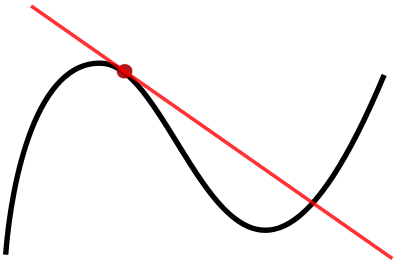
\includegraphics[width=.5\linewidth]{figures/NumericalAndMath/400px-Tangent_to_a_curve.png}
\end{center}
\caption{The graph of a function, drawn in black, and a tangent line to that function, drawn in red. The slope of the tangent line is equal to the derivative of the function at the marked point. (Text from \url{https://en.wikipedia.org/wiki/Derivative} on 2015.05.07; borrowing it because I couldn't find a better way to say it!)}
\end{figure}

\todo{Create a better figure for derivative definition and finite difference, with shown $\Delta x$}

\subsubsection{Partial}

\todo{}

\subsection{Integrals}

Antiderivatives, or integrals, provide the sum of the area under a given curve. These are very useful for solving problems involving processes that occur over space, time, or other (more mathematical, less tangible) dimensions. An example of a non-tangible dimensions would be one that relates to a degree of freedom of some equation and/or error analysis.

\begin{figure}[!ht]
\begin{center}
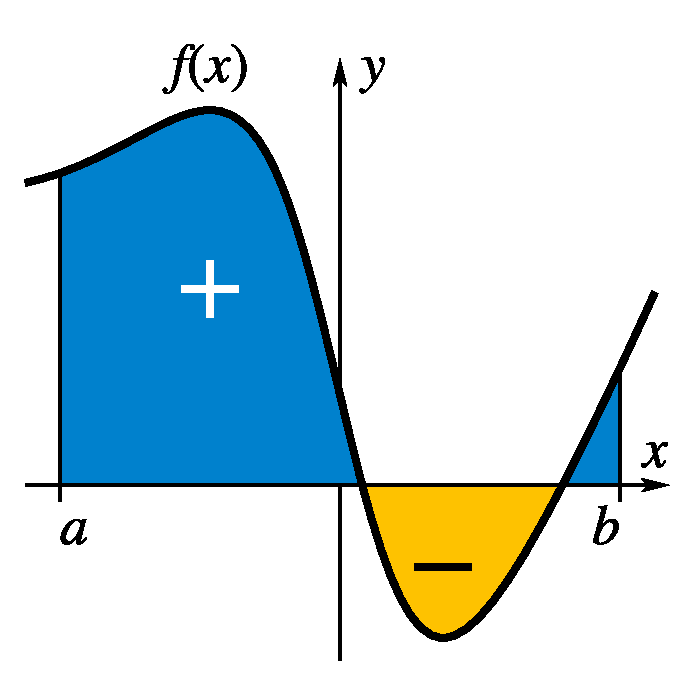
\includegraphics[width=.5\linewidth]{figures/NumericalAndMath/IntegralExample.pdf}
\end{center}
\caption{An integral is the sum of all area under a curve. (Contributed to Wikimedia Commons by User:KSmrq)}
\end{figure}

Indefinite integrals can be defined as:

Definite integrals can be defined as:

\todo{Check}

\begin{equation}
\int_a^b \! f(x)\,dx = F(b) - F(a)
\end{equation}

\begin{equation}
\int_a^b \! f(x)\,dx
\end{equation}

\begin{figure}[!ht]
\begin{center}
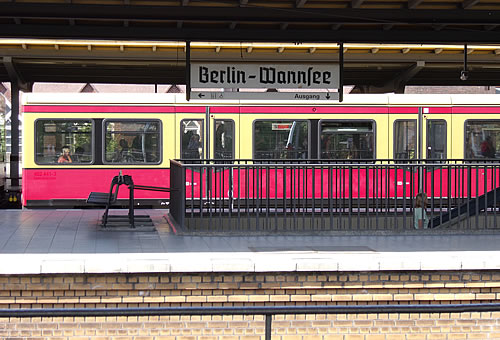
\includegraphics[width=.5\linewidth]{figures/NumericalAndMath/BerlinWannsee.jpg}
\end{center}
\caption{This ``S'' in the Berlin--Wannsee station sign is written in the old style. It is used for integrals to stand for ``sum'', as the area under a curve can be imagined to be a sum $\left( \sum \right)$ of every infinitessimally thin column of space under a curve.}
\end{figure}

\subsection{Taylor series}

The Taylor series of any complex function $f(x)$ (i.e., $f(x) \in \mathbb{C}$) that is infinitely differentiable at a point $x_0$ approximates that function as a power series:
\begin{equation}
f(x_0)+\frac {f'(x_0)}{1!} (x-x_0)+ \frac{f''(x_0)}{2!} (x-x_0)^2+\frac{f^{(3)}(x_0)}{3!}(x-x_0)^3+ \cdots
\end{equation}
Or, in the more-compact summation notation, this is:
\begin{equation}
\sum_{n=0} ^ {\infty} \frac {f^{(n)}(x_0)}{n!} \, (x-x_0)^{n}
\end{equation}
where $n$ is the number of the derivative of $f$.

\begin{figure}[!ht]
\begin{center}
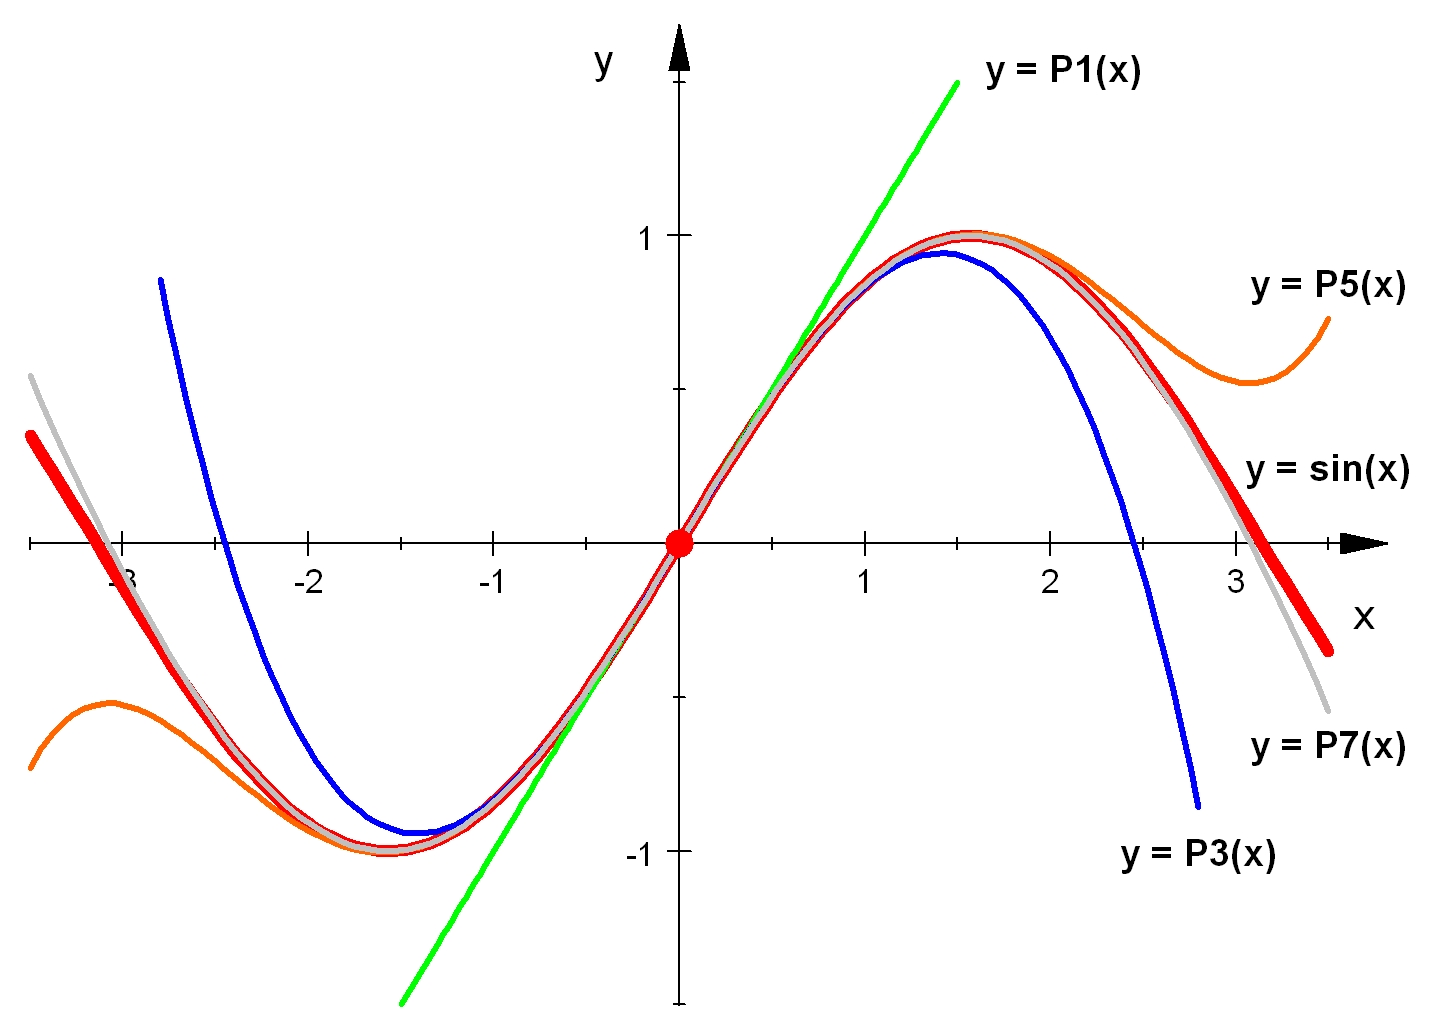
\includegraphics[width=.8\linewidth]{figures/NumericalAndMath/Taylor_Approximation_of_sin(x).jpeg}
\end{center}
\caption{Increasing orders of the Taylor series expansion (and thus its derivative), denoted P$n$, where $n = 1, 2, 3, \cdots$, show the increasing approximation of a sum of polynomials to the sine function.}
\end{figure}

\section{Finite difference}

One of the most useful functions of computers is their ability to approximate the values of derivatives at points. This allow us to directly compute approximations of the values of derivatives in differential equations and therefore solve them, typically through space and/or time.

You may have wondered why I covered derivatives and Taylor series right after one another. This is because these provide two ways to generate finite difference solutions to differential equations. The definition of a derivative provides a way to think of a derivative as the linear tangent to a curve at a given point -- and hence, also, to be well-approximated by a straight line over a finite distance so long as that distance is small compared to the nonlinearity of the curve that it is approximating. This is the same as the second term in the Taylor series expansion.

The Taylor series provides a way to consider higher-order equations that could fit a curve near a certain point. A straight line often is not a poor fit, but if we want to replace an arbitrary function with an infinitely differentiable polynomial, generating a Taylor series approximation is an easy way to do so -- and thus, to numerically solve differential euqations.

The result of this section will be a formalilzation of the \textbf{finite difference method}, by which a set of differential equations is estimated on a grid with constant (but not necessarily uniform) spacings between grid cells (hence finite difference) and then solved. By this, I mean that the distances between grid points stays constant across the varaible over which you are integrating, but may vary with respect to any other variables.

In this class, we will most likey truncate all expansions after the linear first terms: the higher-order terms are more work to include, for both you and the computer, and smaller time-steps or more clever solutiom nethods can often make up for not having them.

\subsection{Where this fits in the spectrum of modeling}

To provide a bit more background, finite difference is just one of several major methods for modeling with continuum equations. Other methods are finite volume (similar to finite difference except considering full cell volume, finite element (which allows a more irregular grid) and spectral (using how something varies in terms of periodic functions in order to write solutions to equations -- this generally requires Fourier and/or other spectral transformations of the equations). Agent-based models that follow the actions of individual ``agets'' in a computational space also exist. These agents are often given simple rules and then allowed to interact with one another.

\subsection{Thermal diffusion}

In the example given here, we will solve the diffusion equation. First, I will present a derivation.

Heat is conducted at a rate that is proportional to the:
\begin{itemize}
 \item \textbf{Temperature difference (directly proportional)}: hotter things more quickly make other things hotter and colder things more quickly make other things colder. The contents of a bottle placed in the freezer will become cold more quickly than will those of one placed in the refrigerator
 \item \textbf{Distance along which heat must be conducted (inversely proportional)}: if there is a thicker wall to a thermos, cooler, or refrigerator, it will better insulate the heat
\end{itemize}
The constant of proportionality, $k$, is called the ``thermal conductivity'' and tells one how easily heat is conducted through a medium. It is an analog to electrical conductivity.

Putting all of these together, we can write (in one dimension):
\begin{equation}
 q_x = -k \frac{d T}{d x}
 \label{eq:FourierThermal}
\end{equation}
Here, $q_x$ is the heat flux (units of Watts per meter squared [W m$^{-2}$]). $x$ indicates that we are solving the equation in the $x$-direction; we will work with a one-dimensional solution here, though you can imagine higher-dimensional solutions to require 2-D instead of 1-D arrays of values for our numerical implementation. The negative sign indicates that heat is flowing downgradient, from hotter items to colder ones.

This expression for thermal conduction (Fourier's Law of Thermal Conduction \todo{check}) can be paired with an expression that describes how the transfer of heat from one object to another results in changes in temperature. This change in temperature produces a \textit{feedback}, by which an object that is conducting heat to another object cools (while the other object warms. This decreases the gradient in temperature between the two objects, and therefore decreases the heat flux.

As one might expect, temperature increases with heat flux into an object and decreases with heat flux out of an object. The negative spatial derivative of heat flux provides the negative divergence (i.e. convergence) of heat at the point of interest. Assuming no phase changes (e.g., solid to liquid), this occurrs at a rate that is inversely proportional to the specific heat capacity of the material and its density.
\begin{equation}
 \frac{\partial T}{\partial t} = -\frac{1}{c_p \rho} \frac{\partial q_x}{\partial x}
 \label{eq:conservation}
\end{equation}

We can plug Equation \ref{eq:FourierThermal} into Equation \ref{eq:conservation} to produce a single equation for thermal conduction
\begin{equation}
 \frac{\partial T}{\partial t} = \frac{1}{c_p \rho} \frac{\partial}{\partial x} \left( k \frac{\partial q_x}{\partial x} \right)
\end{equation}


If we assume that the thermal conductivity, $k$, is spatially uniform, then we can pull it outside the derivative. This yields the most common form of the \emph{diffusion equation}, one of the most widely-used equations in science.
\begin{equation}
 \frac{\partial T}{\partial t} = \frac{k}{c_p \rho} \frac{\partial^2 q_x}{\partial x^2}
\end{equation}
Redefining the coefficients on the right-hand side of the equation as $\kappa$, which is known as ``thermal diffusivity'' and for many Earth materials $\approx 10^{-6}$ m$^2$ s$^{-1}$ yields:
\begin{equation}
 \frac{\partial T}{\partial t} = \kappa \frac{\partial^2 q_x}{\partial x^2}
\end{equation}
In addition to heat transfer, the diffusion equation cab be used to model any process in which a rate is linearly dependent on the difference in values of some state variable. This includes chemical fluxes, temperature fluxes, groundwater flow, hillslope geomorphic change, ...

\subsection{Discretization}

The simplest way to ``discretize'' an equation, or turn it into something that can represent changes over finite (i.e., $\Delta x = \text{ some number } > 0$) distances, is to replace the d$x$ or $\partial x$ terms with a finite $\Delta x$. In doing so, we need to take into account a couple of considerations:
\begin{enumerate}
 \item What do our grids of variables look like?
 \item Do we want to generate differences forwards or backwards in time? (I am focusing on changes in time here, but you can really model a function -- in this case, integrating it numerically -- over any variable.)
\end{enumerate}

\subsubsection{Grids}

For our thermal diffusion example, there are two (or three) important grids, each of which I will represent as a column vector (not to waste space, but to prepare you for matrix methods to be introduced in a later section). The first is our temperatures:
\begin{equation}
 \boldsymbol{T} =
 \begin{bmatrix}
  T_{1} \\
  T_{2} \\
  \vdots \\
  T_{m}
 \end{bmatrix}
\end{equation}

And the second is position:
\begin{equation}
 \boldsymbol{T} =
 \begin{bmatrix}
  x_{1} \\
  x_{2} \\
  \vdots \\
  x_{m}
 \end{bmatrix}
\end{equation}

\subsubsection{Differences}

In order to do finite difference calculations, we must make, well, finite differences! But how should we define our differences? There are a few ways. Using the example of $T(x)$:

\begin{itemize}
 \item Left-handed or ``upwind'' difference scheme:
 \begin{equation}
 1
 \end{equation}
 %\item \frac{dT}{dx} = \frac{T^{
\end{itemize}





\begin{equation}
 \frac{\Delta T}{\Delta t} = \kappa \frac{\partial^2 q_x}{\partial x^2}
\end{equation}



Forward difference and ``implicit''
on both structured and unstructured meshes

Stencils

Linearizing equations (is this the right word? turning them into a set of linear equations)

Differential equations and linear algebra review

Include examples

\section{Example: hillslope diffusion}

This example is from something I wrote for CSDMS, \url{http://csdms.colorado.edu/wiki/Introduction_to_Python}

\subsection{Theory}

Numerical models are fundamentally a computer-readable way to interpret rules that we have provided about how the natural world should work. Here, we are creating a simple model of a hillslope profile with rivers incising on either end. We don't worry about regolith development or any specific hillslope processes. In our case, these rules take the form of partial differential equations. It is extremely important to have a full grasp of and—insofar as it is possible—analytical solution for these equations before beginning.

Here, we make the simple assumption that regolith discharge is a linear function of slope:

\begin{equation}
Q = - k S
\end{equation}

Here, <math>Q</math> is regolith discharge [square meters per year], <math>S</math> is slope [unitless], and <math>k</math> is a constant of proportionality that scales slope to discharge. The negative sign is present because we want positive discharge where there are negative (i.e. downhill) slopes (or, in other words, elevation decreasing as <math>x</math>-distance increases).

We want all of our equations in terms of elevation <math>z</math>, and distance across the hillslope profile, <math>x</math>. Substituting these into <math>S</math> gives us:

\begin{equation}
Q = - k \frac{dz}{dx}
\end{equation}

Hillslope evolution occurs when we combine these discharges to conserve mass. We use a continuity equation for conservation of volume to state that:

\begin{equation}
\frac{\partial z}{\partial t} = - \frac{\partial Q}{\partial x}
\end{equation}

Combining these two terms together gives us the diffusion equation:

\begin{equation}
\frac{\partial z}{\partial t} = \frac{\partial}{\partial x} \left(k \frac{\partial z}{\partial x}\right)
\end{equation}

If we assume that the hillslope diffusivity, <math>k</math>, is uniform across the landscape, we obtain the diffusion equation in its more familiar form:
\begin{equation}
\frac{\partial z}{\partial t} = k \frac{\partial^2 z}{\partial x^2}
\end{equation}

\subsection{Source code}

First, I will write the whole source code. Then I will break it down into sections where I explain each component. Then I will present a new model that uses an implicit matrix-style solution instead of a foward-time-stepping solution, and write about numerical (finite difference) methods.

\begin{lstlisting}[language=Python]
#! /usr/bin/python

# Import modules
import numpy as np
from matplotlib import pyplot as plt

"""
Copyright 2012 Andrew D. Wickert

    This program is free software: you can redistribute it and/or modify
    it under the terms of the GNU General Public License as published by
    the Free Software Foundation, either version 3 of the License, or
    (at your option) any later version.

    This program is distributed in the hope that it will be useful,
    but WITHOUT ANY WARRANTY; without even the implied warranty of
    MERCHANTABILITY or FITNESS FOR A PARTICULAR PURPOSE.  See the
    GNU General Public License for more details.

    You should have received a copy of the GNU General Public License
    along with this program.  If not, see <http://www.gnu.org/licenses/>.
"""

################################################################################
# hill.py
# 
# HILLSLOPE PROFILE
# 
# Center of hill is at 0, two incising channels at steady rate at edges
# no channel-hillslope feedback and assuming entire hill is made of mobile 
# regolith
# 
# This is a very simple example code in which variables are defined inline, 
# and the equations are solved by forward difference methods without 
# consideration for stability
# 
# Written by Andrew D. Wickert; August, 2013
################################################################################

# We will have the simple boundary condition of rivers on either end of the 
# hillslope that are incising at the same, steady rate.
zdot_channel = 2E-4 # [m], 0.5 mm/yr boundary incision

# time
dt = 100. # [years], the time step (from guessing, not from stability analysis)
t_final = 4E5 # [years], the final time for hillslope evolution
timesteps = np.arange(0,t_final + dt/10.,dt) # [years]

# Set up domain
dx = 10 # [m]
xmax = 500 # [m]
x = np.arange(-xmax, xmax + dx/10., dx) # [m], +dx/10. to make sure that edges are included
z = t_final * zdot_channel * np.ones(x.shape) # [m], elevation in meters - set such that the edges are 0 at t_final

# We're using a very simplified assumption that the rate of hillslope 
# material transport is linearly proportional to local slope, and that this 
# constant of proportionality is constant across the hill
k = 5E-3 # Slope -- soil flux scaling

# Loop through time and evolve elevation
for t in timesteps:
  # The channels set the boundaries
  z[0] -= zdot_channel * dt
  z[-1] -= zdot_channel * dt
  # for np.diff, out[n] = a[n+1] - a[n]
  # We are calculating the slopes between each of the cells, then using 
  # these to solve for discharge of material between interior cells.
  S = np.diff(z) # [-] slope
  Q = -k*S # [m**2/yr] discharge, goes downslope, hence the negative sign # POSITIVE - WHY? CANCELLED OUT AGAIN!
  # The change in internal elevation, due to conservation of mass, is equal 
  # once again to the x-defivative
  dzdt_interior = np.diff(Q)
  z[1:-1] -= dzdt_interior * dt
  # (It would have been quicker to take both derivatives at once, but would be 
  # somewhat less intuitive for descriptive purposes)

# Plot
plt.plot(x,z,'k-',linewidth=3)
plt.title('Final hillslope profile', fontsize=20, weight='bold')
plt.xlabel('Distance across hillside [m]', fontsize=16)
plt.ylabel('Elevation [m]', fontsize=16)
plt.xlim((x[0],x[-1]))
plt.show()
\end{lstlisting}

\subsubsection{The ``Shebang''}

This script starts with:
\begin{lstlisting}[language=Python]
#! /usr/bin/python
This is a "shebang" that tells the program where to look for the Python interpreter on Unix-like systems (the most popular being Mac and Linux, the former more popular for desktop applications and the latter more popular for supercomputers). You can find where Python is located by typing:
<syntaxhighlight lang=bash>
which python
\end{lstlisting}
at the Unix command prompt (i.e. terminal).

\subsubsection{Module Import (and Namespaces)}
\begin{lstlisting}[language=Python]
# Import modules
import numpy as np
from matplotlib import pyplot as plt
\end{lstlisting}

Python is a general-purpose language, which means that for specific functionalities, you have to import ''modules''. These modules are sets of functions that share a namespace (''np'' and ''plt'', respectively). '''Numpy''' does general mathematical and ''n''-dimensional array operations, and '''Pyplot''' does basic plotting. "Sharing a namespace" means that to call functions within these modules, we must use the ''np'' and ''plt'' prefixes, e.g., to plot a parabola:

\begin{lstlisting}[language=Python]
a = np.array([[0,1,2,3,4],[0,1,4,9,16]]) # Create an array with 2 rows and 3 columns - nested sets of brackets add dimensions to the array
plt.plot(a[0,:], a[1,:], 'ko-') # Plot the first row of "a" as ''x''-values and the second row as ''y''-values with a dashed line between points
plt.show() # Show the plot in a display screen
\end{lstlisting}

Namespaces are important, because it means that you cannot easily accidentally overwrite the name of a function by giving a variable that name. For example, typing "np.mean = 1.5" seems a less-likely accident than writing "mean = 1.5".

\subsubsection{Copyright Notice}

The aforementioned code is trivial, but lately (2012) it seems that big, ugly patent wars are being fought over trivial chunks of code. So better to be safe than sorry. Below is text included for version 3 of the [http://www.gnu.org GNU] General Public License (GPL). This is an open-source "copyleft" license, meaning that if this code is included in a project, the project must be open-source with a "copyleft" license as well. This is a very good license for science, which is a community-driven collaborative effort. To give your code the GNU GPL v3, include the following text (though replacing my name with yours in the copyright, unless you are feeling generous).

In order for your code to be included in CSDMS, you need to include some type of open-source license, even if it is not as strong a license as the GPL v3.

\begin{lstlisting}[language=Python]
"""
Copyright 2012 Andrew D. Wickert

    This program is free software: you can redistribute it and/or modify
    it under the terms of the GNU General Public License as published by
    the Free Software Foundation, either version 3 of the License, or
    (at your option) any later version.

    This program is distributed in the hope that it will be useful,
    but WITHOUT ANY WARRANTY; without even the implied warranty of
    MERCHANTABILITY or FITNESS FOR A PARTICULAR PURPOSE.  See the
    GNU General Public License for more details.

    You should have received a copy of the GNU General Public License
    along with this program.  If not, see <http://www.gnu.org/licenses/>.
"""
\end{lstlisting}

On a technical note, the triple quotes at the beginning and end of the block are used in Python to create blocks of text as strings. These can be used later inside functions, blocks of code designed for a single purpose, to provide accessible documentation. For now, since we are not assigning this string anywhere, it simply functions as a comment.

\subsubsection{Introductory Comments and Authorship}

This section is huge overkill for this short of a model, but I put it in here to be complete.

\begin{lstlisting}[language=Python]
################################################################################
# hill.py
# 
# HILLSLOPE PROFILE
# 
# Center of hill is at 0, two incising channels at steady rate at edges
# no channel-hillslope feedback and assuming entire hill is made of mobile 
# regolith
# 
# This is a very simple example code in which variables are defined inline, 
# and the equations are solved by forward difference methods without 
# consideration for stability
# 
# Written by Andrew D. Wickert; August, 2013
################################################################################
\end{lstlisting}

\subsubsection{Initialization}

\begin{lstlisting}[language=Python]
# We will have the simple boundary condition of rivers on either end of the 
# hillslope that are incising at the same, steady rate.
zdot_channel = 2E-4 # [m], 0.5 mm/yr boundary incision

# time
dt = 100. # [years], the time step (from guessing, not from stability analysis)
t_final = 4E5 # [years], the final time for hillslope evolution
timesteps = np.arange(0,t_final + dt/10.,dt) # [years]

# Set up domain
dx = 10 # [m]
xmax = 500 # [m]
x = np.arange(-xmax, xmax + dx/10., dx) # [m], +dx/10. to make sure that edges are included
z = t_final * zdot_channel * np.ones(x.shape) # [m], elevation in meters - set such that the edges are 0 at t_final

# We're using a very simplified assumption that the rate of hillslope 
# material transport is linearly proportional to local slope, and that this 
# constant of proportionality is constant across the hill
k = 5E-3 # Slope -- soil flux scaling
\end{lstlisting}

\subsubsection{Main Loop}

\begin{lstlisting}[language=Python]
# Loop through time and evolve elevation
for t in timesteps:
  # The channels set the boundaries
  z[0] -= zdot_channel * dt
  z[-1] -= zdot_channel * dt
  # for np.diff, out[n] = a[n+1] - a[n]
  # We are calculating the slopes between each of the cells, then using 
  # these to solve for discharge of material between interior cells.
  S = np.diff(z) # [-] slope
  Q = -k*S # [m**2/yr] discharge, goes downslope, hence the negative sign # POSITIVE - WHY? CANCELLED OUT AGAIN!
  # The change in internal elevation, due to conservation of mass, is equal 
  # once again to the x-defivative
  dzdt_interior = np.diff(Q)
  z[1:-1] -= dzdt_interior * dt
  # (It would have been quicker to take both derivatives at once, but would be 
  # somewhat less intuitive for descriptive purposes)
\end{lstlisting}

\subsubsection{Plotting}

\begin{lstlisting}[language=Python]
# Plot
plt.plot(x,z,'k-',linewidth=3)
plt.title('Final hillslope profile', fontsize=20, weight='bold')
plt.xlabel('Distance across hillside [m]', fontsize=16)
plt.ylabel('Elevation [m]', fontsize=16)
plt.xlim((x[0],x[-1]))
plt.show()
\end{lstlisting}


\end{document}          
